\documentclass[a4paper]{article}
\usepackage[utf8]{vietnam}
\usepackage[left=3cm,right=2cm,top=2cm,bottom=2cm]{geometry}
\usepackage{amsmath}
\setlength{\parindent}{0pt}
\usepackage{graphicx} 
\usepackage{multirow}
\usepackage{url}
%\usepackage{wallpaper}
%\usepackage[firstpage]{draftwatermark} 
\usepackage{xcolor}
\usepackage{tikz} 
\usepackage{scrextend}
\usepackage{ulem}
\changefontsizes{13pt}
%\usepackage{background}
\usetikzlibrary{calc}
\usepackage{fancyhdr}
\usepackage[sorting=none]{biblatex}
\addbibresource{references.bib}
\usepackage{hyperref}

\usepackage{titlesec}
\usepackage{enumitem}
\usepackage{amsmath}
\titleformat{\section}{\fontsize{13}{15}\selectfont\bfseries}{\thesection}{1em}{}
\titleformat{\subsection}{\fontsize{13}{15}\selectfont\bfseries}{\thesubsection}{1em}{}
\usepackage{enumitem}
%----------------------- config của sy-------------
\usepackage{setspace}
\onehalfspacing
\usepackage{float}
\restylefloat{figure}
\floatplacement{figure}{H}
\usepackage{indentfirst}
\setlength{\parindent}{1cm}
%--------------------------------------Header footer------------------------------------
\pagestyle{fancy}
\fancyhf{} % Xóa định dạng hiện tại của header và footer

% Header
\lhead{Nhóm 2}
\chead{}
\rhead{Ứng dụng GMM phát hiện đối tượng chuyển động trong video}

% Footer
\lfoot{}
\cfoot{} % Hiển thị số trang ở giữa footer
\rfoot{\thepage}

% Định dạng các đường line ở header và footer
\renewcommand{\headrulewidth}{0.1pt} % Độ dày của đường line ở header
\renewcommand{\footrulewidth}{0.1pt} % Độ dày của đường line ở footer
%---------------------------------------------------------------------------------------
%\backgroundsetup{scale = 1, angle = 0, opacity = 0.2,
%contents = {\includegraphics[width = 0.9\paperwidth,
%height = 0.9\paperheight, keepaspectratio] {hust.png}}}

%\backgroundsetup{scale = 1, angle = 0, opacity = 0.2,
%contents = {\includegraphics[width = 0.97\paperwidth,
%height = 0.97\paperheight, keepaspectratio] {bia.png}}}
\begin{document}

\begin{titlepage}
%\SetWatermarkText{\includegraphics[width = 0.97\paperwidth,
%height = 0.97\paperheight]{bia.png}}
%\SetWatermarkAngle{0} 
%\SetWatermarkText{\includegraphics[scale=1]{hust.png}}
%\SetWatermarkAngle{0} 
\begin{tikzpicture}[remember picture,overlay,inner sep=0,outer sep=0]
     \draw[black!80!black,line width=4pt] ([xshift=-2cm,yshift=-2cm]current page.north east) coordinate (A)--([xshift=3cm,yshift=-2cm]current page.north west) coordinate(B)--([xshift=3cm,yshift=2cm]current page.south west) coordinate (C)--([xshift=-2cm,yshift=2cm]current page.south east) coordinate(D)--cycle;

     \draw ([yshift=0.5cm,xshift=-0.5cm]A)-- ([yshift=0.5cm,xshift=0.5cm]B)--
     ([yshift=-0.5cm,xshift=0.5cm]B) --([yshift=-0.5cm,xshift=-0.5cm]B)--([yshift=0.5cm,xshift=-0.5cm]C)--([yshift=0.5cm,xshift=0.5cm]C)--([yshift=-0.5cm,xshift=0.5cm]C)-- ([yshift=-0.5cm,xshift=-0.5cm]D)--([yshift=0.5cm,xshift=-0.5cm]D)--([yshift=0.5cm,xshift=0.5cm]D)--([yshift=-0.5cm,xshift=0.5cm]A)--([yshift=-0.5cm,xshift=-0.5cm]A)--([yshift=0.5cm,xshift=-0.5cm]A);

     \draw ([yshift=-0.3cm,xshift=0.3cm]A)-- ([yshift=-0.3cm,xshift=-0.3cm]B)--
     ([yshift=0.3cm,xshift=-0.3cm]B) --([yshift=0.3cm,xshift=0.3cm]B)--([yshift=-0.3cm,xshift=0.3cm]C)--([yshift=-0.3cm,xshift=-0.3cm]C)--([yshift=0.3cm,xshift=-0.3cm]C)-- ([yshift=0.3cm,xshift=0.3cm]D)--([yshift=-0.3cm,xshift=0.3cm]D)--([yshift=-0.3cm,xshift=-0.3cm]D)--([yshift=0.3cm,xshift=-0.3cm]A)--([yshift=0.3cm,xshift=0.3cm]A)--([yshift=-0.3cm,xshift=0.3cm]A);

   \end{tikzpicture}


\begin{center}
    \vspace{7pt}
    \fontsize{14pt}{16pt}
    \textbf{TRƯỜNG ĐẠI HỌC BÁCH KHOA - ĐẠI HỌC ĐÀ NẴNG}
    
    \vspace{7pt}
    \textbf{KHOA ĐIỆN TỬ - VIỄN THÔNG} \\
    **************************
\end{center}
\vspace{10pt}
\begin{center}
    
\includegraphics[scale=0.37]{images/logodut.jpg}
    
\includegraphics[scale=0.75]{images/logoete.jpg}
    
    \vspace{20pt}
    \fontsize{20pt}{17pt}\selectfont 
    \textbf{BÁO CÁO} \\
    \vspace{7pt}
    \textbf{Học phần: Trí tuệ nhân tạo}
    \vspace{7pt}

\end{center}
\begin{flushleft}
    \fontsize{15pt}{10pt}\selectfont  
    \textbf{\textsl{\hspace{27pt}{\uline{ĐỀ TÀI:}}}}
\end{flushleft}
\begin{center}
    \hspace{10pt}
    \fontsize{17pt}{17pt}\selectfont 
    \textbf{\textrm{Ứng dụng GMM phát hiện đối tượng chuyển động trong video}}
\end{center}
\begin{center}
    \fontsize{16pt}{17pt}\selectfont 
    \textbf{\textrm{}}
\end{center}

\vspace{50pt}
\begin{addmargin}[1cm]{0cm}
\textbf{Giảng viên hướng dẫn: \hspace{2cm}Hoàng Lê Uyên Thục}
\end{addmargin}
\vspace{10pt}
% Bảng sinh viên thực hiện thụt vào 2cm
\begin{addmargin}[1cm]{0cm}
\textbf{Sinh viên thực hiện: \hspace{2.6cm}NHÓM 2}
\begin{tabbing}
\hspace{6cm}\=\hspace{3cm}\=\hspace{3cm} \kill
{\textbf{Họ và tên}}\>{\textbf{MSSV}}\>{\textbf{Mã học phần}}\\
\hspace{6cm}\=\hspace{3cm}\=\hspace{3cm} \kill
Lê Phạm Công\> 106200221\> 20.44\\
\hspace{6cm}\=\hspace{3cm}\=\hspace{3cm} \kill
Phan Công Danh\> 106200222\> 20.44\\
\hspace{6cm}\=\hspace{3cm}\=\hspace{3cm} \kill
Đoàn Thế Lên\> 106200233\> 20.44\\
\hspace{6cm}\=\hspace{3cm}\=\hspace{3cm} \kill
Lê Minh Nhật\> 106200238\> 20.44\\
\end{tabbing}
\end{addmargin}
\vspace{1cm}
\begin{center}
    \textit{\textbf{Đà Nẵng, ngày 31 tháng 05 năm 2024}}
\end{center}
\end{titlepage}
% -------------------------------------End trang bìa-----------------------
\newpage
\tableofcontents
\newpage

% ----------------------- MAIN DOCUMENT---------------------------%
\section*{Tóm tắt}
\addcontentsline{toc}{section}{Tóm tắt}
Trong báo cáo này trình bày một giải pháp sử dụng thuật toán
phân cụm Gaussian Mixture Models để phát hiện đối tượng chuyển động trong video với ý tưởng là phép trừ nền. Trong phương pháp đề xuất, video vào được chuyển đổi thành các frame,
sau đó áp dụng thuật toán Gaussian Mixture Models để phân cụm các điểm ảnh nhằm phân tách nền và các đối tượng sau đó áp dụng phép trừ nền để tìm các đối tượng chuyển động. Kết quả thu được là video chứa các đối tượng chuyển động được phát hiện. 
Mã nguồn của báo cáo có thể được tìm thấy tại: \url{https://drive.google.com/drive/folders/16n3Rrp28noYswsqQs8qazX2qylk2z2YL?usp=sharing}

\section{Giới thiệu}
Trong lĩnh vực xử lý hình ảnh và thị giác máy tính, việc phát hiện chuyển động trong video là một bài toán quan trọng với nhiều ứng dụng như giám sát an ninh, theo dõi đối tượng và phân tích hành vi. Phát hiện chuyển động giúp trích xuất các thông tin hữu ích từ luồng video, đặc biệt là trong các tình huống có thay đổi quan trọng trong cảnh quay.

Gaussian Mixture Models (GMM) là một kỹ thuật mô hình hóa phân phối xác suất, đặc biệt hữu ích trong việc phân loại các điểm dữ liệu phức tạp. Trong lĩnh vực phát hiện chuyển động, GMM được sử dụng để xây dựng mô hình nền của cảnh, từ đó giúp tách biệt các vật thể di chuyển khỏi nền tĩnh. Mô hình này cho phép xử lý các thay đổi trong ánh sáng, tiếng ồn, hoặc chuyển động nhỏ của nền.

Dự án này tập trung vào ứng dụng GMM để phát hiện chuyển động trong các đoạn video. Bằng cách xây dựng một mô hình nền động sử dụng Gaussian Mixture Models, hệ thống có khả năng phân biệt giữa các chuyển động thực sự và các biến đổi không đáng kể của nền, từ đó xác định chính xác khu vực chuyển động.

\section{Phương pháp}
Trong mục này giới thiệu 2 phần, phần 2.1 trình bày về Gaussian Mixture Model (GMM) thông qua ứng dụng với bài toán clustering, phần 2.2 sẽ trình bày việc áp dụng trong việc phát hiện đối tượng chuyển động trong video.

\subsection{Gaussian Mixture Model\cite{gaussian_mixture_python}}
Trong lĩnh vực của các thuật toán unsupervised learning, Gaussian Mixture Model  (GMM) là những thành phần đặc biệt. GMM dựa trên giả định rằng tất cả các điểm dữ liệu đến từ một hỗn hợp tinh tế của phân phối Gaussian với các tham số không biết. Chúng là các mô hình sinh tham số cố gắng học được phân phối dữ liệu thực sự. 

GMM như là sự tổng quát của thuật toán phân cụm K-Means. Giống như K-Means, GMM cũng đòi hỏi số lượng cụm K là đầu vào của thuật toán học. Tuy nhiên, có một sự khác biệt chính giữa hai thuật toán này. K-Means chỉ có thể học được các cụm có hình tròn. Ngược lại, GMM có thể học được các cụm có bất kỳ hình dạng elip nào.

Ngoài ra, K-Means chỉ cho phép một quan sát thuộc về một và chỉ một cụm. Khác biệt, GMM cung cấp các xác suất liên quan đến mỗi ví dụ với một cụm cụ thể. Đối với mỗi quan sát, GMM học các xác suất của ví dụ đó thuộc về mỗi cụm k. Nói chung, GMM cố gắng học mỗi cụm như là một phân phối Gaussian khác nhau. Nó giả định dữ liệu được tạo ra từ một hỗn hợp giới hạn của Gaussians.

Giả định dữ liệu một chiều và số lượng cụm K bằng 3, GMM cố gắng học 9 tham số: 3 tham số cho các giá trị trung bình (mean), 3 tham số cho phương sai (variance), 3 tham số tỷ lệ.

Ở đây, mỗi cụm được biểu diễn bằng một phân phối Gaussian riêng biệt. Đối với mỗi Gaussian, nó học một tham số trung bình và một tham số phương sai từ dữ liệu. 3 tham số tỷ lệ, 1 cho mỗi Gaussian, chỉ được sử dụng cho ước lượng mật độ.

Để học các tham số như vậy, GMM sử dụng thuật toán kỳ vọng tối đa (EM: expectation-aximization) để tối ưu hóa ước lượng hợp lý tối đa. Trong quá trình này, GMM sử dụng Định lý Bayes để tính toán xác suất của một quan sát nhất định $x_i$ thuộc về mỗi cụm k, cho k = 1,2,…, K.

Xem xét một dữ liệu một chiều được tổng hợp. Xây dựng một tập dữ liệu mô phỏng bằng cách lấy mẫu các điểm từ K phân phối Gaussian khác nhau. Mỗi phân phối (với trung bình và phương sai riêng) đại diện cho một cụm khác nhau trong dữ liệu được tổng hợp. Để làm cho mọi thứ rõ ràng hơn, sử dụng K=3:
\begin{equation}
    C_k \sim \mathcal{N}(\mu, \sigma^2)
    \label{eq:normal_distribution}
\end{equation}

Một biến ngẫu nhiên $C_k$ tuân theo phân phối Gaussian được kí hiệu như công thức (\ref{eq:normal_distribution}), trong đó $\mu$ và $\theta$  là hai tham số đặc trưng của phân phối Gaussian. Phân phối Gaussian có hình dạng là một quả chuông mà giá trị xác suất lớn nhất tại $C_k = \mu$ , hình dạng của phân phối đối xứng qua $\mu$. 

Hàm mật độ xác suất (probability density function - pdf) được định nghĩa tại công thức (\ref{eq:normal_pdf}) như sau:
\begin{equation}
    f(x) = \frac{1}{\sqrt{2\pi\sigma^2}} \exp\left(-\frac{(x-\mu)^2}{2\sigma^2}\right)
    \label{eq:normal_pdf}
\end{equation}

Hình \ref{fig:data-and-pdf} Mô tả dữ liệu được sử dụng để học các cụm với GMM. Một số điểm dữ liệu có thể bị chồng chéo với nhau.
\begin{figure}
    \centering
    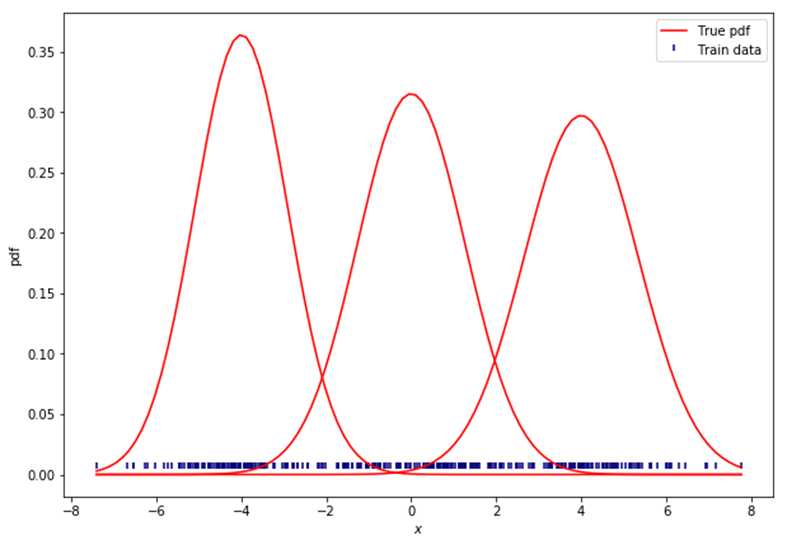
\includegraphics[width=0.7\linewidth]{images/data-and-pdf.png}
    \textit{\caption{Mô tả dữ liệu sẽ sử dụng để học các cụm với GMM.\cite{gaussian_mixture_python}}}
    \label{fig:data-and-pdf}
\end{figure}

Có thể thấy GMM như là một tổng có trọng số của các phân phối Gaussian. Số lượng cụm K xác định số lượng phân phối Gaussian muốn điều chỉnh. Số lượng cụm cần được xác định trước. Số lượng cụm K đã được giả định là 3. Trong tình huống này, GMM sẽ cố gắng học 3 phân phối Gaussian. Đối với dữ liệu một chiều, cần học một tham số trung bình và một tham số phương sai cho mỗi Gaussian.

Trước khi bắt đầu chạy EM, cần đưa ra các giá trị ban đầu cho các tham số có thể học được. Có thể đoán các giá trị cho các trung bình và phương sai, và khởi tạo các tham số trọng số là 1/k. Sau đó, có thể bắt đầu tối ưu hóa hợp lý tối đa bằng cách sử dụng thuật toán EM. EM có thể được đơn giản hóa trong 2 giai đoạn: các bước E (expectation: mong đợi) và M (maximization: tối đa hóa).

Trong bước E, toán xác suất của mỗi quan sát $x_i$ bằng cách sử dụng các tham số ước lượng.
\begin{equation}
    f(x|\mu_k, \sigma_k^2) = \frac{1}{\sqrt{2\pi \sigma_k^2}} \exp\left(-\frac{(x-\mu_k)^2}{2\sigma_k^2}\right)
    \label{eq:conditional_normal_pdf}
\end{equation}
Công thức (\ref{eq:conditional_normal_pdf}) là công thức phân phối Gaussian một chiều (1-D Gaussian distribution) với các tham số:
\begin{itemize}[label={}]
    \item x: là biến ngẫu nhiên theo phân phối Gaussian 
	\item $\mu_k$: trung bình của phân phối
	\item $\theta_k^2$: phương sai của phân phối
\end{itemize}

Đối với mỗi cụm k = 1,2,3,…,K, tính toán mật độ xác suất (pdf) của dữ liệu của chúng ta bằng cách sử dụng các giá trị ước lượng cho trung bình và phương sai. Tại điểm này, những giá trị này chỉ là các dự đoán ngẫu nhiên.

Sau đó, có thể tính toán xác suất của một ví dụ cụ thể $x_i$ thuộc về cụm thứ k như công thức (\ref{eq:posterior_probability}).
\begin{equation}
    b_k = \frac{f(x|\mu_k, \sigma_k^2) \phi_k}{\sum_{k=1}^K f(x|\mu_k, \sigma_k^2) \phi_k}
    \label{eq:posterior_probability}
\end{equation}

Sử dụng Định lý Bayes thu được xác suất hậu nghiệm của phân phối Gaussian thứ k để giải thích dữ liệu. Đó là xác suất mà quan sát $x_i$ được tạo ra bởi phân phối Gaussian thứ k. Lưu ý rằng các tham số $\theta$ đóng vai trò như niềm tin tiên nghiệm của rằng một ví dụ được rút ra từ một trong các phân phối Gaussian đang được mô hình hóa. Vì không có bất kỳ thông tin bổ sung nào để ủng hộ một phân phối Gaussian hơn các phân phối khác nên sẽ bắt đầu bằng cách đoán rằng xác suất là bằng nhau để một ví dụ có thể đến từ mỗi phân phối Gaussian. Tuy nhiên, ở mỗi vòng lặp, cần cải thiện các tiên nghiệm cho đến khi hội tụ.

Sau đó, trong bước tối đa hóa, hoặc bước M, sẽ ước lượng lại các tham số học như công thức (\ref{eq:parameter_updates}):
\begin{equation}
    \begin{aligned}
        \mu_k &= \frac{\sum b_k x}{\sum b_k}, \\
        \sigma_k^2 &= \frac{\sum b_k (x - \mu_k)^2}{\sum b_k}, \\
        \phi_k &= \frac{1}{N} \sum b_k
    \end{aligned}
    \label{eq:parameter_updates}
\end{equation}
Ở đây, cho mỗi cụm, cập nhật trung bình ($\mu_k$), phương sai ($\theta_k^2$), và các tham số tỷ lệ $\phi_k$. Để cập nhật trung bình, cân nhắc mỗi quan sát bằng cách sử dụng xác suất có điều kiện $b_k$.
Cần lặp lại các bước này cho đến khi hội tụ. Điều này có thể đến một điểm nơi các cập nhật tham số nhỏ hơn một ngưỡng dung sai cho trước. Ở mỗi vòng lặp, cập nhật các tham số để giống với phân phối dữ liệu thực sự.

Mở rộng đối với dữ liệu nhiều chiều (D>1), chỉ có một số thay đổi nhỏ. Thay vì ước lượng trung bình và phương sai cho mỗi phân phối Gaussian thì ước lượng trung bình và ma trận hiệp phương sai. Ma trận hiệp phương sai là một ma trận vuông có hình dạng (D, D) trong đó D đại diện cho số chiều của dữ liệu. Tham khảo ví dụ một tập dữ liệu 2-D được sử dụng để điều chỉnh một số lượng hỗn hợp của các phân phối Gaussian khác nhau tại \cite{gaussian_mixture_python}.

\subsection{Ứng dụng Gaussian Mixture Model phát hiện đối tượng chuyển động trong video}
Phương pháp sử dụng mô hình hỗn hợp Gaussian (Gaussian Mixture Model - GMM) để phát hiện vật thể chuyển động trong video được thực hiện thông qua các quá trình sau:
\begin{itemize}[label={}]
    \item 1) Video đầu vào được xử lý bằng thư viện OpenCV để trích xuất các khung hình.
    \item 2) Đối với mỗi vị trí điểm ảnh, giá trị pixel tại vị trí đó được lưu trữ qua tất cả các khung hình trong một mảng và được đưa vào hàm Gaussian Mixture để biểu diễn dưới dạng hỗn hợp của hai phân phối Gaussian.
    \item 3) Một phân phối Gaussian sẽ biểu diễn cho nền (background), và phân phối Gaussian còn lại sẽ biểu diễn cho vật thể nổi bật (foreground) tại vị trí điểm ảnh đó qua tất cả các khung hình.
    \item 4) Vì nền thường giữ nguyên trong hầu hết các khung hình, nên giá trị trung bình của phân phối Gaussian có trọng số lớn hơn và độ lệch chuẩn nhỏ hơn sẽ được sử dụng để xây dựng mô hình nền.
    \item 5) Để theo dõi vật thể, ta trừ mô hình nền này khỏi mỗi khung hình.
\end{itemize}

Cách tiếp cận này sử dụng GMM để mô hình hóa sự biến đổi giá trị pixel tại mỗi vị trí điểm ảnh qua các khung hình trong video. Bằng cách sử dụng hai thành phần Gaussian, nó phân tách được nền tĩnh và vật thể chuyển động. Nền được xây dựng từ thành phần Gaussian có trọng số cao nhất và độ lệch chuẩn thấp nhất. Sau đó, vật thể chuyển động có thể được phát hiện bằng cách trừ nền khỏi mỗi khung hình\cite{background_extraction_video}.

Phương pháp này hiệu quả trong việc phát hiện vật thể chuyển động ngay cả khi có sự thay đổi nhẹ về ánh sáng hoặc nhiễu trong video, vì GMM có khả năng mô hình hóa sự biến đổi này thông qua các phân phối Gaussian.

Thuật toán Gaussian Mixture Model thực hiện việc phát hiện đối tượng chuyển động trong video như sau:
\begin{itemize}[label={}]
    \item Bước 1. Cho dữ liệu đầu vào là giá trị pixel của từng vị trí trên các khung hình trong video.
    \item Bước 2. Giả sử giá trị pixel tại mỗi vị trí được biểu diễn bằng hỗn hợp của hai phân phối Gaussian (một cho nền và một cho vật thể nổi bật).
    \item Bươc 3. Khởi tạo các giá trị trung bình và phương sai ban đầu cho hai phân phối Gaussian.
    \item Bước 4. Tính mật độ xác suất (PDF - Probability Density Function) của từng quan sát (giá trị pixel) theo công thức phân phối Gaussian (\ref{eq:conditional_normal_distribution}).
    \begin{equation}
        f(x|\mu_k, \sigma_k^2) = \frac{1}{\sqrt{2\pi \sigma_k^2}} \exp\left(-\frac{(x-\mu_k)^2}{2\sigma_k^2}\right)
        \label{eq:conditional_normal_distribution}
    \end{equation}
    \item Bước 5: Tính xác suất để một quan sát thuộc về mỗi phân phối Gaussian theo công thức (\ref{eq:posterior_probability}):
    \begin{equation}
        b_k = \frac{f(x|\mu_k, \sigma_k^2) \phi_k}{\sum_{k=1}^K f(x|\mu_k, \sigma_k^2) \phi_k}
        \label{eq:posterior_probability}
    \end{equation}
    \item Bước 6. Sử dụng định lý Bayes để tính xác suất hậu nghiệm (posterior probability) của mỗi Gaussian, cho biết xác suất mà quan sát được sinh ra từ phân phối đó.
    \item Bước 7. Cập nhật các tham số (trung bình, phương sai, trọng số) cho các phân phối Gaussian dựa trên xác suất hậu nghiệm.
    \begin{equation}
        \begin{aligned}
            \mu_k &= \frac{\sum b_k x}{\sum b_k}, \\
            \sigma_k^2 &= \frac{\sum b_k (x - \mu_k)^2}{\sum b_k}, \\
            \phi_k &= \frac{1}{N} \sum b_k
        \end{aligned}
        \label{eq:parameter_updates}
    \end{equation}
    \item Bước 8. Lặp lại quá trình cho đến khi các giá trị trung bình, phương sai và trọng số hội tụ.
\end{itemize}
\newpage
\section{Kết quả}
Dữ liệu được sử dụng là video được quay bởi camera giám sát giao thông, thông số video như sau: thời lượng 30s, kích thước khung hình 1920x1080pixels, tốc độ khung hình 25fps. Đường dẫn đến dữ liệu: \url{https://drive.google.com/file/d/1BXUZeLSU-4lmNtu7ZnffGqG2RwKMkNBU/view?usp=sharing}

Kết quả thử nghiệm với video dữ liệu như sau: 
\begin{itemize}[label={}]
    \item 1) Ảnh nền
    \begin{figure}
        \centering
        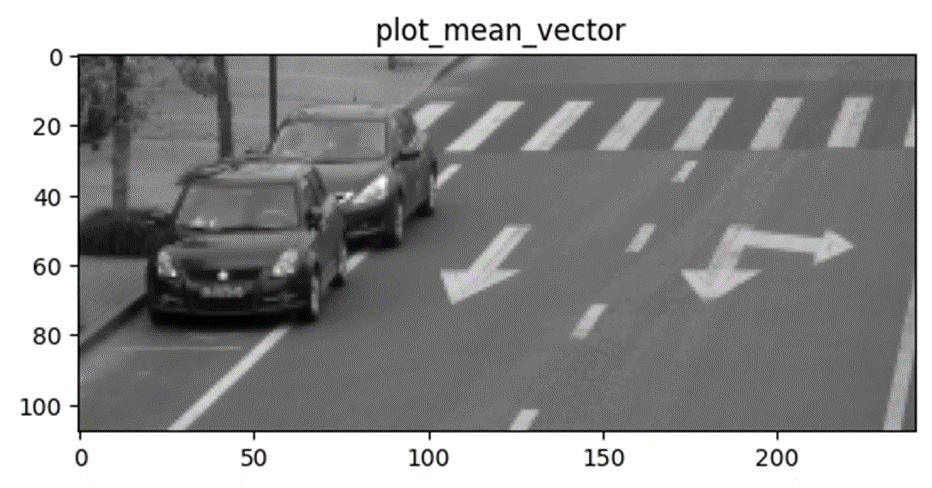
\includegraphics[width=0.7\linewidth]{images//result/background.png}
        \label{fig:background}
        \textit{\caption{Ảnh nền}}
    \end{figure}
    \item 2) Một số frame sau khi thực hiện phép trừ nền (tất cả frame được lưu trữ lại folder frame) như bảng \ref{fig:answer}
    \begin{table}
        \centering
        \textbf{\caption{Kết quả của phép trừ nền trên một số frame}}
        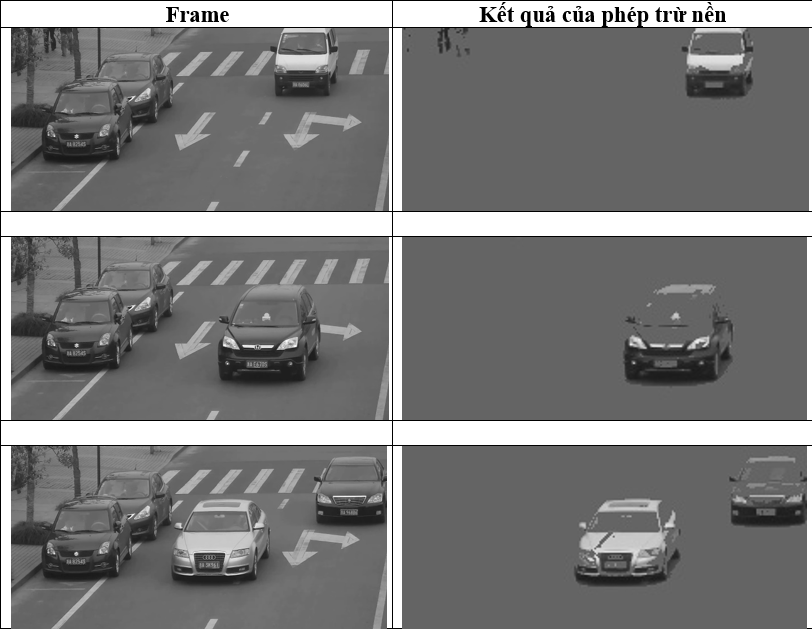
\includegraphics[width=0.75\linewidth]{images//result/result3.png}
        \label{fig:answer}
    \end{table}
    \\ \\ \\ \\ \\ \\ \\ \\ \\ \\ \\ \\ \\ \\ \\ \\ 
    \item 3) Video kết quả: \url{https://youtu.be/2Ktw_daaETQ}
    \item 4)  Độ chính xác: Các khung hình đầu ra được tính toán bằng thuật toán được so sánh với các khung hình đầu ra thu được sau khi sử dụng hàm BackgroundSubtractorMOG2 dựng sẵn trong OpenCV2. Số liệu được sử dụng cho so sánh là MSE\cite{mean_squared_error}. Các khung hình từ thuật toán được xây dựng chỉ được chuyển đổi sang màu đen và trắng cho so sánh công bằng vì hàm dựng sẵn chỉ cung cấp các khung đầu ra có màu đen và trắng. Giá trị lớn nhất RMSE thu được là 86,37 và RMSE tối thiểu thu được là 3.17 
    \item 5) Histogram của MSE (hình \ref{fig:mse}):
    \begin{figure}
        \centering
        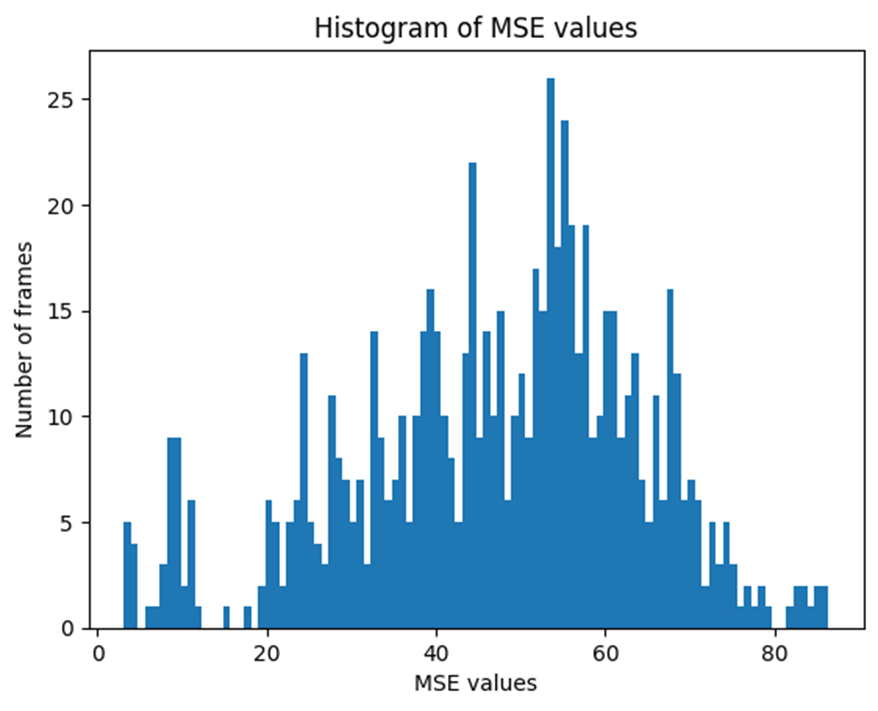
\includegraphics[width=1\linewidth]{images//result/mse.png}
        \caption{Histogram của MSE}
        \label{fig:mse}
    \end{figure}
    \item 6) So sánh với thuật toán được xây dựng và sử dụng thư viện Opencv như bảng 2:
    \begin{table}
        \centering
        \textbf{\caption{So sánh kết quả phép trừ nền giữa thuật toán được xây dựng và hàm có sẵn trong thư viện}}
        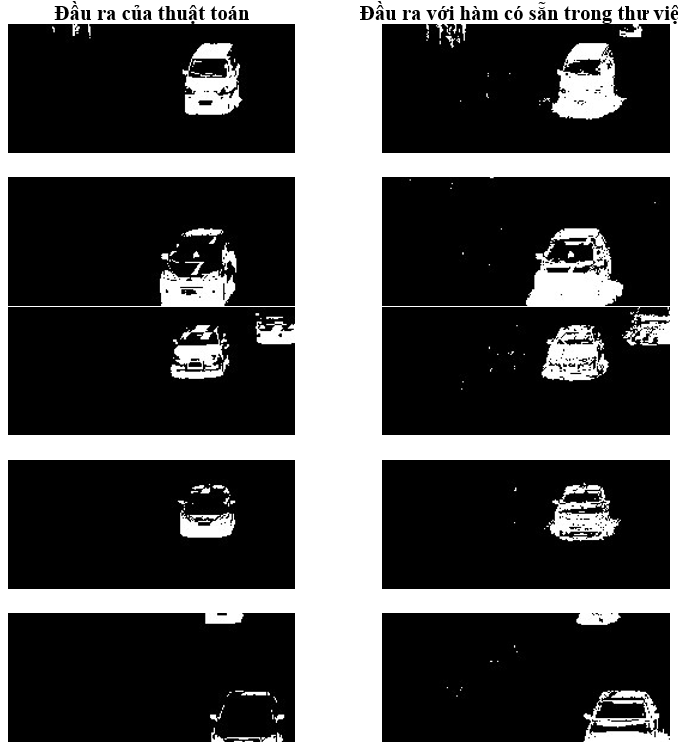
\includegraphics[width=1\linewidth]{images//result/sosanh.png}
        \label{fig:so-sanh}
    \end{table}
\end{itemize}
\newpage
\section{Đánh giá}
Đầu tiên, thuật toán đã xác định đúng ảnh nền, đây là bước quan trọng đảm bảo phép trừ nền thực hiện chính xác hay không, nếu không xác định đúng nền, có thể dẫn đến kết quả cuối cùng không chính xác.

Thứ hai, phép trừ nền mang lại kết quả tương đối, một số chi tiết bị mất, nguyên nhân là do một số chi tiết có màu trùng với màu nền hoặc chất lượng video đầu vào không tốt vẫn còn nhiễu nên các chi tiết đó bị trùng với nền.

Thứ ba, kết quả trong video đầu ra là các đối tượng được cho là đang chuyển động trong video, dựa vào video kết quả có thể nhận thấy, thuật toán đã detect thành công các đối tượng chuyển động trong video với sự hỗ trợ của Gaussian Mixture Model

Thứ tư, giá trị lớn nhất RMSE thu được là 86,37 và RMSE tối thiểu thu được là 3.17. Giá trị MSE cao chỉ ra rằng có một sự chênh lệch đáng kể giữa hình ảnh dự đoán và hình ảnh thực tế trong một số trường hợp cụ thể, ở đây là giữa việc sử dụng thuật toán tự xây dựng và thư viện hỗ trợ. Giá trị MSE thấp cho thấy thuật toán hoạt động tốt trong một số khung hình, với sự chênh lệch ít giữa hình ảnh dự đoán và hình ảnh thực tế. Điều này có thể xảy ra trong các điều kiện lý tưởng nơi nền tương đối đơn giản và ít nhiễu, hoặc khi các đối tượng chuyển động có đường nét rõ ràng. Thông qua việc xem xét chi tiết các trường hợp khi RMSE đạt giá trị cao nhất và thấp nhất để tìm ra cách để tối ưu hóa thuật toán và cải thiện độ chính xác của nó trong các tình huống khác nhau.

\section{Kết luận}
Việc sử dụng mô hình Gaussian Mixture (GMM) để phát hiện đối tượng chuyển động trong video là một phương pháp phổ biến và có hiệu quả, nhất là trong các ứng dụng giám sát video và an ninh. Dưới đây là một số điểm mạnh và hạn chế của phương pháp này, cùng với một số kết luận về hiệu quả của nó:
Điểm Mạnh:
\begin{itemize}[label={}]
    \item 1) Phân biệt Nền và Đối tượng: GMM giỏi trong việc phân biệt giữa nền tĩnh và đối tượng chuyển động bằng cách mô hình hóa mỗi điểm ảnh như một hỗn hợp của nhiều phân phối Gaussian. Điều này cho phép nó phát hiện chuyển động ngay cả trong các điều kiện ánh sáng phức tạp.
    \item 2) Cập nhật Động: Mô hình có thể được cập nhật theo thời gian để thích ứng với các thay đổi trong cảnh, như sự thay đổi của điều kiện ánh sáng hoặc biến động nền mới.
    \item 3) Hiệu quả với Nhiều Đối tượng: GMM có khả năng phát hiện nhiều đối tượng chuyển động cùng một lúc, điều này là hữu ích cho các ứng dụng giám sát đông đúc.
\end{itemize}
Hạn Chế:
\begin{itemize}[label={}]
    \item 1)Nhạy cảm với Nhiễu: Mặc dù GMM có thể thích ứng với các thay đổi trong video, nó vẫn có thể nhạy cảm với nhiễu, nhất là trong điều kiện ánh sáng yếu hoặc khi có sự chuyển động của bụi hoặc lá cây.
    \item 2) Tính toán Tốn kém: Việc ước tính và cập nhật các tham số Gaussian cho mỗi điểm ảnh có thể rất tốn kém về mặt tính toán, đặc biệt là với video độ phân giải cao và trong thời gian thực.
    \item 3)Thiếu Ổn định trong Môi trường Động: Trong các cảnh có sự thay đổi nền liên tục, GMM có thể mất nhiều thời gian để thích ứng, dẫn đến các phát hiện sai hoặc bỏ sót.
\end{itemize}

Tóm lại, mô hình Gaussian Mixture là một công cụ mạnh mẽ để phát hiện đối tượng chuyển động trong video, nhờ khả năng mô hình hóa chính xác và thích ứng với sự thay đổi của nền. Tuy nhiên, tính hiệu quả của nó có thể bị ảnh hưởng trong các điều kiện nhiễu hoặc động. Để tối đa hóa hiệu quả, các nhà phát triển và nhà nghiên cứu nên cân nhắc kết hợp GMM với các kỹ thuật khác như bộ lọc nhiễu, phân tích điểm khóa, hoặc sử dụng nó trong một khuôn khổ học sâu nâng cao để giải quyết các hạn chế về nhiễu và tốn kém tính toán. Các cải tiến này có thể giúp GMM trở thành một giải pháp hiệu quả hơn cho các ứng dụng giám sát video và an ninh hiện đại.


%---------------------REFERENCES --------------------------------%
\newpage
\renewcommand*{\bibfont}{\small}
\printbibliography

\end{document}

